\documentclass[onecolumn]{article}
\usepackage{array,booktabs,bytefield}
\usepackage{graphicx, here}
\begin{document}

\pagenumbering{roman}

\title{ALSA control interface design}
\author{Takashi Sakamoto}
\date{2015/05/01}
\maketitle{}

\begin{abstract}

Linux Advanced Sound Architecture

\end{abstract}

\section*{Acknowledgement}

hoge

\newpage

\tableofcontents

\newpage

\pagenumbering{arabic}

\section{Introduction}

\section{ALSA Control Component}

ALSA includes some components corresponds to each functionality of actual sound devices\footnote{alsa-firewire-report}. One of the components is responsible for control functionality. I reffer it to Control Component in this document.

In this section, I describe the Control Component.

\subsection{Element, Element set, channels and dimension}

In ALSA, each card instance\footnote{struct snd\_card} has a role as a Control Component, thus each driver has no need to add specific instances for the component.

\begin{figure}[htbp]
	\centering
	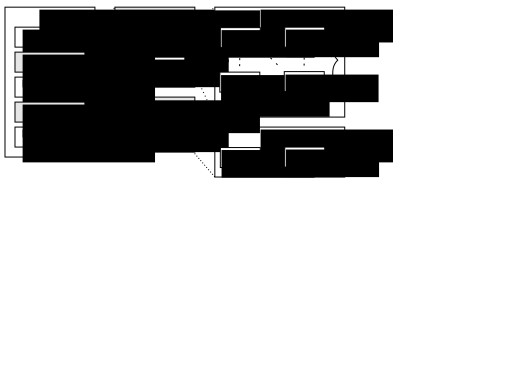
\includegraphics[scale=0.75]{./img/alsa-control-model.svg.eps}
	\caption{{ALSA Control component model}}
	\label{fig:alsa-control-model}
\end{figure}

Each controllable substance of actual card is represented as an element. Each driver adds some instances of element, then, corresponding card instance manages the instances in a linked-list.

The instance can includes several elements with the same feature. To distinguish the instance from single element, I describe it as element set. The element set is added by one operation and includes several element indicated by one of function parameters. Elements in the same element set have the similar features indicated by one of the function parameters..

One element consists of several channels. One channel has its own controllable value, thus one channel is corresponding to a register or a part of register. The maximum number of channel which one element can include is determined by type of the element.

Usually, the channels are handled as one array. The two neiboughr channel represents the neighbour registers or two part of registers. On the other hand, the element has dimension to handle matrix value. When an element has the dimension info, for example two dimension, the channel array represents two dimention matrix.


\subsection{Element addressing}

When added to card instance, each element gain unique numerical number from the card. There're two ways to identify each element in the element set. One is just to use the numerical number, another is to use a combination of some parameters with element name.

The name of elements is the same as the name of the element set. To distinguish these elements, numerical number, index is used.

Each driver can allow to add element set with the same name. In this case, these element sets are added with the value of index for the first element in each element set so as no overlap index for the elements with the same name.

To use the name and the index for identification, the other parameters are also required. They're interface, device and subdevice. 6 types of the interface are defined; card, hwdep, mixer, pcm, rawmidi, timer and sequencer. The mixer interface is used for usual elements, while one of the other interfaces is used when the element set is closely associated with a corresponding component such as PCM. In this case, the device and subdevice are also used to indicate the assosiated components\cite{alsa-driver}.

The identical information is transferred with the same structure, 'struct snd\_ctl\_elem\_id'\footnote{include/uapi/sound/asound.h in Linux kernel source code}. See Figure \ref{fig:control-element-id}. As described above, there is no need to fill all of the members.

\begin{figure}[htbp]
\small
\begin{verbatim}
#define SNDRV_CTL_ELEM_ID_NAME_MAXLEN	44

struct snd_ctl_elem_id {
    unsigned int numid;
    snd_ctl_elem_iface_t iface;
    unsigned int device;
    unsigned int subdevice;
    unsigned char name[SNDRV_CTL_ELEM_ID_NAME_MAXLEN];
    unsigned int index;
};
\end{verbatim}
\caption{{Structure of identical information for control element}}
\label{fig:control-element-id}
\end{figure}


\subsection{Element set information}

Element set can have basic information. When adding new element set, each driver gives the information.

Each element includes several channels. Originally, the channels in an element are used to represent controlable substance in the same register. Currently the channel is used regardless of the actual register.

There're 7 types of element; boolean, bytes, integer, integer64, iec958 and enumerated. See Figure \ref{fig:element-set-types}. The boolean, bytes, integer and integer64 element has the corresponding type of value for its channels. The iec958 element includes flags to describe parameters for IEC 60958. The enumerated element has several labels to describes labeled values.

\begin{figure}[htbp]
\small
\begin{verbatim}
#define SNDRV_CTL_ELEM_TYPE_BOOLEAN     1
#define SNDRV_CTL_ELEM_TYPE_INTEGER     2
#define SNDRV_CTL_ELEM_TYPE_ENUMERATED  3
#define SNDRV_CTL_ELEM_TYPE_BYTES       4
#define SNDRV_CTL_ELEM_TYPE_IEC958      5
#define SNDRV_CTL_ELEM_TYPE_INTEGER64   6
\end{verbatim}
\caption{{Types of element set}}
\label{fig:element-set-types}
\end{figure}

The integer and integer64 element has a constrain of range for its value of each channel. Additionally, it has the value of step for its discretion.

In the enumerated element, the length of each label is restricted by 63 characters (64 bytes with terminator) and the length of total labels is limited by 64 * 1024 bytes including their terminators.

The information is represented by 'struct snd\_ctl\_elem\_info'\footnote{include/uapi/sound/asound.h}. See Figure \ref{fig:element-set-info-structure}. This structure is used by each drivers to set information for element.

\begin{figure}[htbp]
\small
\begin{verbatim}
struct snd_ctl_elem_info {
    struct snd_ctl_elem_id id;
    snd_ctl_elem_type_t type;
    unsigned int access;
    unsigned int count;
    __kernel_pid_t owner;
    union {
        struct {
            long min;
            long max;
            long step;
        } integer;
        struct {
            long long min;
            long long max;
            long long step;
        } integer64;
        struct {
            unsigned int items;
            unsigned int item;
            char name[64];
            __u64 names_ptr;
            unsigned int names_length;
        } enumerated;
        unsigned char reserved[128];
    } value;
    union {
        unsigned short d[4];
    } dimen;
    unsigned char reserved[64-4*sizeof(unsigned short)];
};
\end{verbatim}
\caption{{Structure for control element set information}}
\label{fig:element-set-info-structure}
\end{figure}

The dimen member includes dimention information. In detail, I describe in later section.

\subsection{Channel values for element}

As described, element can include several channels. The maximum number of channels included in an element depends on the type of element. See Table \ref{tbl:max-channels}

\begin{table}[H]
        \centering
        \caption{{The maximum number of channels for each element}}
        \label{tbl:max-channels}
        \begin{tabular}{ccc} \toprule
		type & maximum \\ \midrule
		boolean & 128 \\
		byte & 512 \\
		integer & 128 \\
		integer64 & 64 \\
		iec958 & 1 \\
		enumerated & 128 \\ \bottomrule
        \end{tabular}
\end{table}

The limitation comes from structure for these values. See Figure \ref{fig:element-channel-value}. In ALSA core, the value for boolean, enumerated type is represented by the same way as integer, thus they have the same maximum number, 128.

This structure can deliver timestamp information when these values are read or changed, while actual implementation depends on driver side.

\begin{figure}[htbp]
\small
\begin{verbatim}
struct snd_ctl_elem_value {
    struct snd_ctl_elem_id id;
    union {
        union {
            long value[128];
        } integer;
        union {
            long long value[64];
        } integer64;
        union {
            unsigned int item[128];
        } enumerated;
        union {
            unsigned char data[512];
        } bytes;
        struct snd_aes_iec958 iec958;
    } value;
    struct timespec tstamp;
    unsigned char reserved[128-sizeof(struct timespec)];
};
\end{verbatim}
\caption{{Channel value of a control element }}
\label{fig:element-channel-value}
\end{figure}


\subsection{Element channel dimension for matrix}

Some devices has multiplxer, which multiplexes several source signals to one sink signal. When devices have several multiplexers for a corresponding number of sinks from the same number of sources, typically, controllable parameters consists of source-sink matrix.

ALSA drivers can use element channels to represent the matrix, then optional information is required for the number of sources and the number of sinks. For this purpose, element channel dimension is used.

The element channel dimension has an array of 4 members of unsigned short type, thus it can describe maximum 4 dimensions. Total number of columns in the matrix is calculated by a product of all members of the array, and the number must be within the number of channels of each element type.

Usually, 2 dimensional channel is used for source-sink matrix. In this case, first member of the array has the number of sources, and second member of the array has the number of sinks.

As of Linux 4.01, a part of drivers for devices produced by Echo Digital Audio uses the element channel dimension. Therefore, most devices set zero for each member in this array.


\subsection{Element access type}

Element has its own access type. The access type consists of some flags. See Figure \ref{fig:element-access-flags}. When adding a new element set to card instance, each driver gives the flags as well as the other parameters. All elements in an element set basically have the same flags.

Usually, the controlable substance is readable and writable, thus both of read and write flags are used. If an element allows to handle threshold level, some tlv flags are used. When an element set is added by userspace driver, user flag is used.

The timestamp flag means the read data includes timestamp at which channels of the element are changed. The volatile flag means the channel of element can be asynchronously changed.

\begin{figure}[htbp]
\small
\begin{verbatim}
#define SNDRV_CTL_ELEM_ACCESS_READ          (1<<0)
#define SNDRV_CTL_ELEM_ACCESS_WRITE         (1<<1)
#define SNDRV_CTL_ELEM_ACCESS_READWRITE     (SNDRV_CTL_ELEM_ACCESS_READ |
                                             SNDRV_CTL_ELEM_ACCESS_WRITE)
#define SNDRV_CTL_ELEM_ACCESS_VOLATILE      (1<<2)
#define SNDRV_CTL_ELEM_ACCESS_TIMESTAMP     (1<<3)
#define SNDRV_CTL_ELEM_ACCESS_TLV_READ      (1<<4)
#define SNDRV_CTL_ELEM_ACCESS_TLV_WRITE     (1<<5)
#define SNDRV_CTL_ELEM_ACCESS_TLV_READWRITE (SNDRV_CTL_ELEM_ACCESS_TLV_READ |
                                             SNDRV_CTL_ELEM_ACCESS_TLV_WRITE)
#define SNDRV_CTL_ELEM_ACCESS_TLV_COMMAND   (1<<6)
#define SNDRV_CTL_ELEM_ACCESS_INACTIVE      (1<<8)
#define SNDRV_CTL_ELEM_ACCESS_LOCK          (1<<9)
#define SNDRV_CTL_ELEM_ACCESS_OWNER         (1<<10)
#define SNDRV_CTL_ELEM_ACCESS_TLV_CALLBACK  (1<<28)
#define SNDRV_CTL_ELEM_ACCESS_USER          (1<<29)
\end{verbatim}
\caption{{Element access flags}}
\label{fig:element-access-flags}
\end{figure}

These flags tell implementation requirements to userspace applications. For example, when an element has read flag, userspace applications can execute read operation to the element. Of cource, each driver should have corresponding implementation.

Basically, some flags in a element is mutable, while the inactive, lock and owner flags are immutable to describe current status of the element. The inactive flag means the element exists but is not activated. The combination of lock and owner flags means the locking state of element.


\subsection{Locking state of element}

An userspace application can lock arbitrary elements. The process to lock the element is called as 'owner'. When locked, the other processes can read channels of the element, while cannot write to channels of the element.

In locking state, when reading information of the element, it has lock flag. When the owner process read the information, the element has lock and owner flag.

For both owner process and non-owner process, the information includes owner's PID. In unlocking state, a element gives -1 for the PID field in information data.


\subsection{Threshold level representation and operation for sound pressure}

Generally, in human perception, the maximum and minimum signal level which human can perceive as sound are limited. The perceptived sound is calles as loudness and its level is not linearly increased even if the signal level is linearly increased. Additionally, the loudness level differs depending on signal frequency. There's a series of study about this\footnote{i.e. ISO 226:2003}.

In acoustics engineering, common logarithm\footnote{Logarithm based on 10.} is used for a formula between signal level and loudness level. This way is too primitive and rough, but a simple, easy and practical. In this way, the loudness level is referred to 'sound pressure level', calculated by equation \ref{eq:decibel}.

\begin{equation}
L_p = 10 \log_{10} \frac{p}{p_0} \label{eq:decibel}
\end{equation}

Here, $L_p$ is sound pressure level (decibell, dB), p is measured sound pressure(Pa), $p_0$ is minimum sound pressure level and defined with $2 \times 10^-5$ (Pa).

In most sound devices, corresponding sound drivers control the sound pressure by reading/writing their registers. The driver developers cannot know actual sound pressure, but can know maximum and minimum value on the registers. If incrementing the value of registers can linearly increase the sound pressure, there're some demands for application developer to calculate read/write value according to sound pressure level. Then, some tlv parameters should be given, such as the required value change to change pressure level by a unit of 0.1 dB.

ALSA Control Component refers the threshold level as 'tlv' and gives a way to transfer tlv parameters.

Originally, ALSA Control Component allows each driver to have pre-defined tlv information. This implements one tlv information to each driver instance and allows applications to read the information.

The tlv information is represented by an array consists of unsigned int elements and  has hierarchic structure. The data is capculated by container. Each container has a type in its first element, and the number of included data in its second element. There's just one type of container, SNDRV\_CTL\_TLVT\_DB\_SCALE.

<TODO: graphic>

In 2006, tlv operations are expanded\footnote{commit 8aa9b586e42099817163aba01d925c2660c4dbbe in Linux kernel source code}. Write and command operations were added. Later, new types of container were added.

According to these implementation, each driver can have flexible information for tlv. On the other hand, as if Linux 4.1, no kernel-land drivers supports the command operation.


\subsection{Control event notification}

ALSA Control Component supports event notification. As of Linux 4.1, events for elements are supported. The supported events are removing, changing information, changing the value of channels and handling tlv information.

\begin{figure}[htbp]
\small
\begin{verbatim}
enum sndrv_ctl_event_type {
    SNDRV_CTL_EVENT_ELEM = 0,
    SNDRV_CTL_EVENT_LAST = SNDRV_CTL_EVENT_ELEM,
};

#define SNDRV_CTL_EVENT_MASK_VALUE  (1<<0)
#define SNDRV_CTL_EVENT_MASK_INFO   (1<<1)
#define SNDRV_CTL_EVENT_MASK_ADD    (1<<2)
#define SNDRV_CTL_EVENT_MASK_TLV    (1<<3)
#define SNDRV_CTL_EVENT_MASK_REMOVE (~0U)
\end{verbatim}
\caption{{Defined events}}
\label{defined-events}
\end{figure}

The events for elements are transferred with identical information and event mask.


\section{Driver implementation}

ALSA Control Component has both of kernel API and userspace API.

\subsection{Kernel-land driver}

When adding a new element set, ALSA kernel-land drivers call 'struct snd\_ctl\_new1()' with a template. The template is represented by 'struct snd\_kcontrol\_new'.

\begin{figure}[htbp]
\small
\begin{verbatim}
struct snd_kcontrol_new {
    snd_ctl_elem_iface_t iface;
    unsigned int device;
    unsigned int subdevice;
    const unsigned char *name;
    unsigned int index;
    unsigned int access;
    unsigned int count;
    snd_kcontrol_info_t *info;
    snd_kcontrol_get_t *get;
    snd_kcontrol_put_t *put;
    union {
        snd_kcontrol_tlv_rw_t *c;
        const unsigned int *p;
    } tlv;
    unsigned long private_value;
};
\end{verbatim}
\caption{{Template structure for control element}}
\label{control-element-template}
\end{figure}

This structure includes enough members to build an instance of element set. Four operations are defined as a callback functions.

\begin{description}
\small
\item[snd\_kcontrol\_info\_t] \mbox{} \\
For detail information about the element set
\item[snd\_kcontrol\_get\_t] \mbox{} \\
For get operation of the element set
\item[snd\_kcontrol\_put\_t] \mbox{} \\
For put operation of the element set
\item[snd\_kctl\_tlv\_rw\_t] \mbox{} \\
For threshold level operation of the element set
\end{description}

In info callback function, each driver should fill enough members of passed 'struct snd\_ctl\_elem\_info'. This is mandatory.

In get callback function, each driver is expected to fill current values of corresponding controllable substance. This should be implemented when the element has SNDRV\_CTL\_ELEM\_ACCESS\_READ.

In put callback function, each driver is expected to control corresponding controllable substance by the values of given elements. This should be implemented when the element has SNDRV\_CTL\_ELEM\_ACCESS\_WRITE.

In tlv callback function, each driver can modify its own tlv information or keep/handle given tlv information in the tlv union. This should be implemented when the element has SNDRV\_CTL\_ELEM\_ACCESS\_TLV\_CALLBACK. In this case, the element can have SNDRV\_CTL\_ELEM\_ACCESS\_TLV\_READ, SNDRV\_CTL\_ELEM\_ACCESS\_TLV\_WRITE, SNDRV\_CTL\_ELEM\_ACCESS\_TLV\_COMMAND and the driver can implement corresponding processing.

Instead of implementing tlv callback function, each driver can have old-fascioned, read-only tlv information in the tlv union. In this case, the element should have just SNDRV\_CTL\_ELEM\_ACCESS\_TLV\_READ.

The added element sets are deleted when the device is removed or the driver is unloaded.


\subsection{User-land driver}

ALSA control interface allows userspace applications to add/replace/remove arbitrary element sets into registered card instances. The operation is implemented in ioctl(2) commands. In this document, the userspace application is called as an user-land driver.

\begin{figure}[htbp]
\small
\begin{verbatim}
#define SNDRV_CTL_IOCTL_ELEM_ADD        _IOWR('U', 0x17, struct snd_ctl_elem_info)
#define SNDRV_CTL_IOCTL_ELEM_REPLACE    _IOWR('U', 0x18, struct snd_ctl_elem_info)
#define SNDRV_CTL_IOCTL_ELEM_REMOVE     _IOWR('U', 0x19, struct snd_ctl_elem_id)
\end{verbatim}
\caption{{ioctl(2) commands to handle control element set in userspace}}
\label{ioctl-commands-userspace-element}
\end{figure}

When adding a new element set, userspace driver passes information with identical information and basic parameters. In this operation, the owner field is used for a different purpose. The given value to owner field is used for the number of elements in this element set. The count field is used for the number of channels which an element in this element set has.

Just after added, the element set is under locking. Before unlocking, the driver can set tlv information by write operation. If registering tlv information, SNDRV\_CTL\_ELEM\_ACCESS\_TLV\_WRITE should be given to the information. In this case, the elements automatically has SNDRV\_CTL\_ELEM\_ACCESS\_TLV\_CALLBACK for an internal reason of ALSA core. To allow the other applications to read tlv information, the element set should have SNDRV\_CTL\_ELEM\_ACCESS\_TLV\_READ. For architecture reason, read operations and command operation returns the same result, thus SNDRV\_CTL\_ELEM\_ACCESS\_TLV\_COMMAND has no specific meaning.

The userspace driver should listen to control notification to catch value change of each channel in element.

The remove ioctl is used to remove an element set identified by the given information. I note that these added element set can be also removed by the other applications. Additionally, when no applications remove these element set, they exist till the target card is removed.


\section{ALSA Control Interface for elements}

ALSA Control interface is designed to basic operations such as open(2)/ioctl(2)/read(2)/close(2). Their entry point is a special file for ALSA Control character device.

When opening one of the chracter devices and get a file descriptor, userspace applications can handle elements via the file descriptor. These operations are defined as ioctl(2) commands.

\begin{figure}[htbp]
\small
\begin{verbatim}
#define SNDRV_CTL_IOCTL_ELEM_LIST _IOWR('U', 0x10, struct snd_ctl_elem_list)
#define SNDRV_CTL_IOCTL_ELEM_INFO _IOWR('U', 0x11, struct snd_ctl_elem_info)
#define SNDRV_CTL_IOCTL_ELEM_READ _IOWR('U', 0x12, struct snd_ctl_elem_value)
#define SNDRV_CTL_IOCTL_ELEM_WRITE _IOWR('U', 0x13, struct snd_ctl_elem_value)
#define SNDRV_CTL_IOCTL_ELEM_LOCK _IOW('U', 0x14, struct snd_ctl_elem_id)
#define SNDRV_CTL_IOCTL_ELEM_UNLOCK _IOW('U', 0x15, struct snd_ctl_elem_id)
#define SNDRV_CTL_IOCTL_SUBSCRIBE_EVENTS _IOWR('U', 0x16, int)
#define SNDRV_CTL_IOCTL_TLV_READ _IOWR('U', 0x1a, struct snd_ctl_tlv)
#define SNDRV_CTL_IOCTL_TLV_WRITE _IOWR('U', 0x1b, struct snd_ctl_tlv)
#define SNDRV_CTL_IOCTL_TLV_COMMAND _IOWR('U', 0x1c, struct snd_ctl_tlv)
\end{verbatim}
\caption{{ioctl(2) commands to handle control element}}
\label{ioctl-handle-element}
\end{figure}

\subsection{Element list operation}

Userspace applications can get the list of identical informations of existed element.

\begin{figure}[htbp]
\small
\begin{verbatim}
struct snd_ctl_elem_list {
	unsigned int offset;
	unsigned int space;
	unsigned int used;
	unsigned int count;
	struct snd_ctl_elem_id __user *pids;
	unsigned char reserved[50];
};
\end{verbatim}
\caption{{Structure for control element list}}
\label{snd-ctl-elem-list}
\end{figure}

There're two ways to use this operation. The first way is to get the number of element. When the space field is zero, the count field is filled with the number of element.

Another way is to get the list of indentical informations for existed element. In this case, the pids field has a pointer for pre-allocated memory to identical information list, and the space field is filled with the number of allocated memory at unit of identical information structure.

To avoid allocating excess memory object in kernel space, the maximum number of space is limited within 16384. If there're more element, the offset fields can be available to indicate an offset from the first element with minimum numerical number.

\subsection{Element lock/unlock operation}

The lock operation is used by userspace applications to own a element. The unlock operation is used to release the element. If the element is owned by the other userspace applications, the unlock operation fails.

\subsection{Element event notification and subscription}

If userspace applications want to receive element event notification, the application should call the subscribe events operation in advance. Then, these notification can be readable from a file descriptor.

\begin{figure}[htbp]
\small
\begin{verbatim}
struct snd_ctl_event {
    int type;
    union {
        struct {
            unsigned int mask;
            struct snd_ctl_elem_id id;
        } elem;
        unsigned char data8[60];
    } data;
};
\end{verbatim}
\caption{{Structure for control notification event}}
\label{snd-ctl-event}
\end{figure}

\subsection{Element write/read/command operations for threshold level information}

When the element has corresponding flags, tlv write/read/command operations are available. The structure for this information is 'struct snd\_ctl\_tlv'. See Figure \ref{fig:snd-ctl-tlv}.

\begin{figure}[htbp]
\small
\begin{verbatim}
struct snd_ctl_tlv {
    unsigned int numid;
    unsigned int length;
    unsigned int tlv[0];
};
\end{verbatim}
\caption{{Structure for threashold level information}}
\label{fig:snd-ctl-tlv}
\end{figure}

The 'numid' member is for addressing a control element. The 'length' member is for the length of 'tlv' member. The contents of 'tlv' member is described in Section (TODO).

\subsection{Element info operation}

Info operation is successfull for all of elements. If this information includes some wrong data, it's a fault to develop device driver. All of data in this information should be valid.

\subsection{Element read/write operation}

When an element has SNDRV\_CTL\_IOCTL\_ELEM\_READ, element read operation is available. When the element has SNDRV\_CTL\_IOCTL\_ELEM\_WRITE, element write operation is available. In both operations, the array of channel values in an element is passed. The channels values should be parsed according to the channel dimension.


\section{ALSA library}

ALSA project develops an userspace library to wrap interface differences depending on Linux kernel version and to give higher abstructions for each interfaces such as PCM or Sequencer. In this section, I describe about basic design of ALSA library and control API.


\subsection{Configuration space and plugins}

ALSA interface consists of Control, PCM, Compress\footnote{Currently ALSA library doesn't support this interface.}, RawMidi, Sequencer, Timer and Hardware Dependent (HwDep). They have its own character devices. The main purpose of ALSA library is to capsulate raw access to character deivces and to add software functional implementation to the access.

These functionalities are based on control node in application runtime. This is called as configuration space. The configuration space is based on ALSA configuration files\footnote{/usr/share/alsa/alsa.conf.d/*, /etc/asound.conf and ~/.asoundrc}. These configuration files describe node settings for each interfaces.

When userspace applications open handles for ALSA interfaces, ALSA library parses these configuration files to construct configuration space. Userspace applications can open handlers against the nodes.

Each node setting can have plugin entry. The plugin is to extend node functionality with software implementation. For ALSA Control Interface, hw and shm plugin are included in ALSA library.

The hw plugin execute raw access to ALSA Control character device. The shm plugin is designed for interprocess communication.


\subsection{External control plugins}

ALSA library allows to develop plugins externally. This is called as external control plugin. As of alsa-plugins 1.0.29, arcam, maemo, oss and pulse plugins are included.

The external control plugin can be available by the same way as control plugins in ALSA library.


\subsection{Control API}

Control API is designed to use a handler, 'struct snd\_ctl\_t' for operation. The handler is an opaque pointer for struct \_snd\_ctl\footnote{src/control/control\_local.h} and userspace applications cannot refer to each member of the structure.

\begin{figure}[htbp]
\small
\begin{verbatim}
struct _snd_ctl {
    void *open_func;
    char *name;
    snd_ctl_type_t type;
    const snd_ctl_ops_t *ops;
    void *private_data;
    int nonblock;
    int poll_fd;
    struct list_head async_handlers;
};
\end{verbatim}
\caption{{Control handler internals}}
\label{control-handler-internals}
\end{figure}

The 'type' member means the type of plugin to which the handler is assigend. As of ALSA library 1.0.29, four types are defined, while INET type has no actual plugin implementation.

\begin{figure}[htbp]
\small
\begin{verbatim}
typedef enum _snd_ctl_type {
    SND_CTL_TYPE_HW,
    SND_CTL_TYPE_SHM,
    SND_CTL_TYPE_INET,
    SND_CTL_TYPE_EXT
} snd_ctl_type_t;
\end{verbatim}
\caption{{Types of handlers}}
\label{snd-ctl-type-t}
\end{figure}

When opening the handler, userspace applications call snd\_ctl\_open() with the name of node and a mode flag. As of ALSA library 1.0.29, there're three types of handler mode flags. As of ALSA library 1.0.29 and Linux kernel 4.1, there're no implementation for write operation, therefore readonly flag has no actual effects.

\begin{figure}[htbp]
\small
\begin{verbatim}
#define SND_CTL_NONBLOCK    0x0001
#define SND_CTL_ASYNC       0x0002
#define SND_CTL_READONLY    0x0004
\end{verbatim}
\caption{{Handler flags}}
\label{handler-flags}
\end{figure}

\begin{figure}[htbp]
\small
\begin{verbatim}
typedef struct _snd_ctl snd_ctl_t;
int snd_ctl_open(snd_ctl_t **ctl, const char *name, int mode);
int snd_ctl_open_lconf(snd_ctl_t **ctl, const char *name, int mode,
                       snd_config_t *lconf);
int snd_ctl_open_fallback(snd_ctl_t **ctl, snd_config_t *root, const char *name,
                          const char *orig_name, int mode);
int snd_ctl_close(snd_ctl_t *ctl);
\end{verbatim}
\caption{{Handler operations}}
\label{handler-operations}
\end{figure}

Control API is designed to use opaque pointers for fundamental structures. Thus, userspace applications cannot directrly refer to each members in the structure. Applications use setter and getter functions to touch these members, such as snd\_ctl\_elem\_id\_set\_device() or snd\_ctl\_elem\_info\_is\_writable().

\begin{figure}[htbp]
\small
\begin{verbatim}
typedef struct _snd_ctl_elem_id snd_ctl_elem_id_t;
typedef struct _snd_ctl_elem_list snd_ctl_elem_list_t;
typedef struct _snd_ctl_elem_info snd_ctl_elem_info_t;
typedef struct _snd_ctl_elem_value snd_ctl_elem_value_t;
typedef struct _snd_ctl_event snd_ctl_event_t;
\end{verbatim}
\caption{{Opaque pointers for fundamental structures}}
\label{fig:opaque-pointers}
\end{figure}

To enable each plugin to handle operations, wrapper functions are implemented. The actual processings are depending on plugins.

\begin{figure}[htbp]
\small
\begin{verbatim}
int snd_ctl_elem_list(snd_ctl_t *ctl, snd_ctl_elem_list_t *list);
int snd_ctl_elem_info(snd_ctl_t *ctl, snd_ctl_elem_info_t *info);
int snd_ctl_elem_read(snd_ctl_t *ctl, snd_ctl_elem_value_t *value);
int snd_ctl_elem_write(snd_ctl_t *ctl, snd_ctl_elem_value_t *value);
int snd_ctl_elem_lock(snd_ctl_t *ctl, snd_ctl_elem_id_t *id);
int snd_ctl_elem_unlock(snd_ctl_t *ctl, snd_ctl_elem_id_t *id);
int snd_ctl_elem_tlv_read(snd_ctl_t *ctl, const snd_ctl_elem_id_t *id,
                          unsigned int *tlv, unsigned int tlv_size);
int snd_ctl_elem_tlv_write(snd_ctl_t *ctl, const snd_ctl_elem_id_t *id,
                           const unsigned int *tlv);
int snd_ctl_elem_tlv_command(snd_ctl_t *ctl, const snd_ctl_elem_id_t *id,
                             const unsigned int *tlv);
\end{verbatim}
\caption{{Element operations}}
\label{fig:element-operations}
\end{figure}

Control event notification is also available as long as the plugins support. To get file descriptors for multiplexed I/O operations, getter functions are available. Then subscriber applications can get the notification by executing snd\_ctl\_read() or read(2) system-call.

\begin{figure}[htbp]
\small
\begin{verbatim}
int snd_ctl_poll_descriptors_count(snd_ctl_t *ctl);
int snd_ctl_poll_descriptors(snd_ctl_t *ctl, struct pollfd *pfds,
                             unsigned int space);
int snd_ctl_poll_descriptors_revents(snd_ctl_t *ctl, struct pollfd *pfds,
                                unsigned int nfds, unsigned short *revents);
int snd_ctl_subscribe_events(snd_ctl_t *ctl, int subscribe);
int snd_ctl_read(snd_ctl_t *ctl, snd_ctl_event_t *event);
int snd_ctl_wait(snd_ctl_t *ctl, int timeout);
\end{verbatim}
\caption{{Read-related operations}}
\label{fig:read-related-operations}
\end{figure}

Signal-driven I/O operations is also available as long as plugins implement it.

\begin{figure}[htbp]
\small
\begin{verbatim}
int snd_ctl_nonblock(snd_ctl_t *ctl, int nonblock);
int snd_ctl_abort(snd_ctl_t *ctl);
int snd_async_add_ctl_handler(snd_async_handler_t **handler, snd_ctl_t *ctl, 
			snd_async_callback_t callback, void *private_data);
snd_ctl_t *snd_async_handler_get_ctl(snd_async_handler_t *handler);
\end{verbatim}
\caption{{Asynchronous operations}}
\label{fig:async-operations}
\end{figure}


\subsection{Setup control API}

Setup control API gives a way to control arbitrary elements according to given runtime configuration. This API is originally designed for hook PCM plugin, to set PCM-related controls during playbacking/recording PCM substreams.


\subsection{High level control API}

Well-implemented control applications handle control events and maintain control elements. High level control API is for these works.

The handle of this API is a wrapper of handler for Control API and represented by a specific structure. This handler includes a link-list and an array for hctl elements. The link-list is used to maintain hctl elements and the array is used to sort hctl elements. There're some functions to query these hctl elements.

The hctl elements are represented by a specific structure to wrap each control element. This structure can have a handler to receive notification after handling the event inner library. And the structure has weight parameter for sorting.

These two structures are not public to application, thus applications are allowed to handle them as opaque pointers and should use helper functions to access members of the structure..

The control events are handled inner the library to manage local list for hctl elements. Applications can register its own notification handler. As of Linux 4.01, 'add' event is just passed to the notification handler.

Additionally, each hctl element can also has notification handler and applications can register it. As of Linux 4.01, 'remove', 'value' and 'info' events are passed to the notification handler.

When adding any hctl elements, the local list is refreshed with sorted hctl elements. The default algorithm is snd\_hctl\_set\_compare(). The default algorithm is based on element addressing information and weight from the name. Applications can register an arbitrary functions for the algorithm.

There're two helper functions for event handling; snd\_hctl\_wait() and snd\_hctl\_handle\_events(). They execute poll(2) and read(2) internally. When applications implement them, get descriptors and execute system-calls.


\subsection{Mixer API}

The purpose of mixer API is to give helper functions to control elements with typical usage such as playback and capture, volume and switch. Originally, this API is designed as a wrapper for high level control interface. Later, this wrapper got loadable shared object to handle control elements, and applications can select them as abstraction backend. Currently, four types of backends are available; high level control, AC'97. High definition audio(hda) and python. As of ALSA library version 1.0.29, hda and python backend is still half-implemented\footnote{And the python scripts are written with Python2}.

Applications call snd\_mixer\_selem\_register() with parameters to load each backend. The parameter is represented in 'struct snd\_mixer\_selem\_regopt'. This function check members of the structure and calls snd\_mixer\_selem\_none\_register() or snd\_mixer\_simple\_basic\_register().

\begin{figure}[htbp]
\small
\begin{verbatim}
enum snd_mixer_selem_regopt_abstract {
    SND_MIXER_SABSTRACT_NONE = 0,
    SND_MIXER_SABSTRACT_BASIC,
};

struct snd_mixer_selem_regopt {
    int ver;
    enum snd_mixer_selem_regopt_abstract abstract;
    const char *device;
    snd_pcm_t *playback_pcm;
    snd_pcm_t *capture_pcm;
};
\end{verbatim}
\caption{{Structure for backend options}}
\label{fig:mixer-selem-regopt}
\end{figure}

The 'none' backend is for an bstraction of high level control. This backend is included in libasound2.so binary. The 'basic' backend is to load the other backends according to smixer.conf and the value of 'structure snd\_card.components'. These backends are represented by 'struct \_snd\_mixer\_class'. This structure has

\begin{figure}[htbp]
\small
\begin{verbatim}
struct _snd_mixer_class {
    struct list_head list;
    snd_mixer_t *mixer;
    snd_mixer_event_t event;
    void *private_data;
    void (*private_free)(snd_mixer_class_t *class);
    snd_mixer_compare_t compare;
};
\end{verbatim}
\caption{{Structure for backends}}
\label{fig:mixer-class}
\end{figure}

Each backend has own event handler. This handler is called internally when handling hctl event. When the handler is called with 'add' event, each module keeps an instance of 'struct \_snd\_mixer\_elem' by calling snd\_mixer\_elem\_new().

\begin{figure}[htbp]
\small
\begin{verbatim}
struct _snd_mixer_elem {
    snd_mixer_elem_type_t type;
    struct list_head list;
    snd_mixer_class_t *class;
    void *private_data;
    void (*private_free)(snd_mixer_elem_t *elem);
    snd_mixer_elem_callback_t callback;
    void *callback_private;
    bag_t helems;
    int compare_weight;
};
\end{verbatim}
\caption{{Structure for backends}}
\label{fig:mixer-elem}
\end{figure}

When keep the instance, the function add the instance to link-list in 'struct \_snd\_mixer', which is an handler of mixer API.

\begin{figure}[htbp]
\small
\begin{verbatim}
struct _snd_mixer {
    struct list_head slaves;
    struct list_head classes;
    struct list_head elems;
    snd_mixer_elem_t **pelems;
    unsigned int count;
    unsigned int alloc;
    unsigned int events;
    snd_mixer_callback_t callback;
    void *callback_private;
    snd_mixer_compare_t compare;
};
\end{verbatim}
\caption{{Structure for mixer handler}}
\label{fig:mixer-handler}
\end{figure}

Each element is identified by 'struct \_snd\_mixer\_selem\_id'; the combination of name and index.

\begin{figure}[htbp]
\small
\begin{verbatim}
struct _snd_mixer_selem_id {
    char name[60];
    unsigned int index;
};
\end{verbatim}
\caption{{Mixer element identification}}
\label{fig:mixer-selem-id}
\end{figure}

For applications, these structures are hidden by opaque pointers. Mixer API includes halper functions to access these members.

\begin{figure}[htbp]
\small
\begin{verbatim}
typedef struct _snd_mixer_class snd_mixer_class_t;
typedef struct _snd_mixer_elem snd_mixer_elem_t;
typedef struct _snd_mixer snd_mixer_t;
typedef struct _snd_mixer_selem_id snd_mixer_selem_id_t;
\end{verbatim}
\caption{{Opaque structure for mixer API}}
\label{fig:mixer-opaque-structures}
\end{figure}

When opening the handler, applications call snd\_mixer\_open(). When closing, call snd\_mixer\_close(). Applications attach hctl handler to the mixer handler by calling snd\_mixer\_attach() with control node name. All of control elements are added to the mixer handler by calling snd\_mixer\_load(), then these elements are sorted by comparison function in the mixer handler. When applications call snd\_mixer\_free(), these elements are removed from the mixer handler. For event polling, snd\_mixer\_wait() is available. If applications need to implement poll loop, snd\_mixer\_poll\_descriptors(), snd\_mixer\_poll\_descriptors\_count() and snd\_mixer\_poll\_descriptors\_revents() are available.

To retrieve first element in the link-list, applications call snd\_mixer\_first\_elem(). For last element, use snd\_mixer\_last\_elem(). To iterate the elements, use snd\_mixer\_elem\_next() and snd\_mixer\_elem\_prev(). To seek an element, use snd\_mixer\_find\_selem() with identification information.

These elements are classified to two categories; direction (global/playback/capture) and feature(volume/switch/enumerated). The direction means effective range of the control. The feature means behaviour of the control. Therefore, a mixer element has a internal expression for capability of combinations between these two categories.

\begin{figure}[htbp]
\small
\begin{verbatim}
#define SM_CAP_GVOLUME		(1<<1)
#define SM_CAP_GSWITCH		(1<<2)
#define SM_CAP_PVOLUME		(1<<3)
#define SM_CAP_PVOLUME_JOIN	(1<<4)
#define SM_CAP_PSWITCH		(1<<5)
#define SM_CAP_PSWITCH_JOIN	(1<<6)
#define SM_CAP_CVOLUME		(1<<7)
#define SM_CAP_CVOLUME_JOIN	(1<<8)
#define SM_CAP_CSWITCH		(1<<9)
#define SM_CAP_CSWITCH_JOIN	(1<<10)
#define SM_CAP_CSWITCH_EXCL	(1<<11)
#define SM_CAP_PENUM		(1<<12)
#define SM_CAP_CENUM		(1<<13)
\end{verbatim}
\caption{{Defined capability flags for mixer element}}
\label{fig:mixer-element-capability}
\end{figure}

The 'join' means that all of channels included the mixer control are combined to move. The 'excl' means that the mixer element is a part of mixer element group and one of them is available\footnote{Actuallythis flag is meaningless because ALSA lib has a lack of related implementation.}.

Each mixer element has a set of value corresponding to the number of channels, as control element has. In mixer API, these values are represented as corresponding role. The usual roles are defined as 9 types: front left, front right, rear left, rear right, front center, woofer, side left, side right, rear center.

\begin{figure}[htbp]
\small
\begin{verbatim}
typedef enum _snd_mixer_selem_channel_id {
	SND_MIXER_SCHN_UNKNOWN = -1,
	SND_MIXER_SCHN_FRONT_LEFT = 0,
	SND_MIXER_SCHN_FRONT_RIGHT,
	SND_MIXER_SCHN_REAR_LEFT,
	SND_MIXER_SCHN_REAR_RIGHT,
	SND_MIXER_SCHN_FRONT_CENTER,
	SND_MIXER_SCHN_WOOFER,
	SND_MIXER_SCHN_SIDE_LEFT,
	SND_MIXER_SCHN_SIDE_RIGHT,
	SND_MIXER_SCHN_REAR_CENTER,
	SND_MIXER_SCHN_LAST = 31,
	SND_MIXER_SCHN_MONO = SND_MIXER_SCHN_FRONT_LEFT
} snd_mixer_selem_channel_id_t;
\end{verbatim}
\caption{{Defined IDs for each channels}}
\label{fig:mixer-selem-channel-id}
\end{figure}

To check status of the retrieved element, use snd\_mixer\_selem\_is\_xxx() such as snd\_mixer\_selem\_is\_active(). To check the retrieved element has a certain feature, use snd\_mixer\_selem\_has\_xxx() function series such as snd\_mixer\_selem\_has\_playback\_volume(). To convert between linear value and logarithmic value, use snd\_mixer\_selem\_ask\_xxx() such as snd\_mixer\_selem\_ask\_playback\_dB\_vol().

To get the value of a channel, use snd\_mixer\_selem\_get\_xxx() functions such as snd\_mixer\_selem\_get\_playback\_volume(). Especially, there're 'all' type of set function such as snd\_mixer\_selem\_set\_capture\_switch\_all().


\subsection{Use Case Manager}

\section{Issues}

Setup Control API doesn't handle INTEGER64 element.

Hctl header has no snd\_hctl\_async.

\begin{thebibliography}{99}

\addcontentsline{toc}{section}{References}

\bibitem{alsa-driver}
Writing an ALSA Driver (2005, Takashi Iwai) \\
http://www.alsa-project.org/main/index.php/ALSA\_Driver\_Documentation

\bibitem{}
Enhancement of ALSA firewire stack (2015, Takashi Sakamoto) \\
https://github.com/takaswie/alsa-firewire-report

\end{thebibliography}

\newpage

\appendix

\addcontentsline{toc}{section}{Appendices}
\addtocontents{toc}{\protect\setcounter{tocdepth}{-1}}

\section{hoge}

\section{fuga}

\end{document}
